\begin{appendices}
\chapter{Appendix}
\label{cha:Appendix}

\section{Literature Review Further Content}
\label{sec:Literature Review Further Content}

\subsection{Gipps 1981 Equations}
\label{subsec:Gipps 1981 Equations}
Gipps' 1981 car-following model paper \citep{Gipps1981} defines two equations, which provide constraints on the speed of vehicle $n$ at time $t + \tau$. $t$ is the current time and $\tau$ is the apparent reaction time, a constant for all vehicles. The first equation defines the acceleration constraint of the vehicle. It was obtained using measurements from an instrumented car.

\begin{equation}\label{Gipps1981Accel}
v_n(t+\tau) \leqslant v_n(t) + 2.5a_n\tau\Biggl(\frac{1 - v_n(t)}{V_n}\Biggr)\Biggl(\frac{0.025 + v_n(t)}{V_n}\Biggr)^{1/2}
\end{equation}

$v_n(t)$ is the speed of vehicle $n$ at time $t$. $a_n$ is the maximum acceleration the driver of vehicle $n$ wishes to undertake. $V_n$ is the target speed for vehicle $n$. The equation shows that the driver accelerates until close to their target speed. Then, they reduce their acceleration until it reaches zero. At this point the vehicle should be travelling at it's target speed.

The second constraint is the braking profile of the vehicle. This is given as

\begin{equation}\label{Gipps1981Brake}
\begin{split}
&v_n(t+\tau) \leqslant \\
&b_n\tau + \sqrt{\Biggl(b_n^2\tau^2 - b_n\biggl(2\Bigl[x_{n-1}(t) - s_{n-1} - x_n(t)\Bigr] - v_n(t)\tau - \frac{v_{n-1}(t)^2}{\hat{b}}\biggr)\Biggr)}
\end{split}
\end{equation}

$b_n$ is the most severe braking the driver of vehicle $n$ wishes to undertake. It is always a negative value, and should be considered negative acceleration. $\hat{b}$ is the driver of vehicle $n$'s best guess at $b_{n-1}$ where $n-1$ is $n$'s predecessor. $x_n(t)$ is the location of the front of vehicle $n$ at time $t$. $s_n$ is the effective size of vehicle $n$. This is equal to the physical length of $n$, plus a margin $n$'s successor is not willing to enter, even when $n$ is at rest.

Therefore, at time $t + \tau$, assuming the driver travels as fast as is safe, and within the limitations of the vehicle, their speed is given by the minimum of these two equations.

\begin{equation}
v_n(t) = \min{(\eqref{Gipps1981Accel},\eqref{Gipps1981Brake})}
\end{equation}

\subsection{The Intelligent Driver Model}
\label{subsec:The Intelligent Driver Model}
In 2000 Treiber et al. suggested the 'Intelligent Driver Model' (IDM) \citep{Treiber2000}. In the IDM, the acceleration of vehicle $\alpha$, $\dot{v_\alpha}$, is defined using a continuous function of its velocity, $v_\alpha$; the distance to the rear of its predecessor, $s_\alpha$; and the velocity difference of $\alpha$ and it's predecessor, also known as the approaching rate $\Delta v_\alpha$. The vehicle interactions are solely based on $\alpha$'s relative acceleration to its predecessor. The model only provides position information for a vehicle in relation to its predecessor, and it does not provide its velocity at a given time, as Gipps' model does. 

The IDM is broken into two components. The first describes the behaviour of a vehicle on a free road.

\begin{equation}
\dot{v_\alpha} = a^{(\alpha)}\Biggl[1 - \biggl(\frac{v_\alpha}{v_0^{(\alpha)}}\biggr)^\delta\Biggr]
\end{equation}

Here $a^{(\alpha)}$ is the maximum acceleration of vehicle $\alpha$ and $v_0^{\alpha}$ is the desired velocity of $\alpha$. $\delta$ is the acceleration exponent, which is typically 4. 

The second component describes the behaviour of a vehicle as it approaches its predecessor. 

\begin{equation}
\dot{v_\alpha} = - a^{(\alpha)}\biggl(\frac{s^*}{s_\alpha}\biggr)^2
\end{equation}

As the gap, $s_\alpha$, between $\alpha$ and it's predecessor, gets closer to the desired minimum gap $s^*$, $\alpha$ decelerates.

Interpolating the two components gives us the IDM. 

\begin{equation}
\dot{v_\alpha} = a^{\alpha}\Biggl[1 - \biggl(\frac{v_\alpha}{v_0^\alpha}\biggr)^\delta - \biggl(\frac{s^*(v_\alpha,\Delta v_\alpha)}{s_\alpha}\biggr)^2\Biggr]
\end{equation}

The desired minimum gap in the IDM varies dynamically with velocity and approaching rate. It is given by the following function.

\begin{equation}\label{IDMSpacingFunction}
s^*(v,\Delta v) = s_0^{(\alpha)} + s_1^{(\alpha)}\sqrt{\frac{v}{v_0^{(\alpha)}}} + T^\alpha v + \frac{v\Delta v}{2\sqrt{a^{(\alpha)}b^{(\alpha)}}}
\end{equation}

The equation takes the bumper-to-bumper space $s_0^{(\alpha)}$, also known as the minimum jam distance, and adds the comfortable jam distance $s_1^{(\alpha)}$. The bumper-to-bumper space is the minimum gap between $\alpha$ and its predecessor in stationary traffic. The comfortable jam distance is an extra distance added on for comfort, and to allow for a slower driver reaction time. In the paper, this value is set to $0$. We can also consider it negligible for autonomous vehicles. $T$ is the safe time headway; it represents the time required for the vehicle to safely come to a stop. Finally $b^{(\alpha)}$ is the desired deceleration for $\alpha$.

\subsection{Atagoziyev's Model}
\label{sec:Atagoziyev's Model}

In the paper SV (subject vehicle) refers to the vehicle that wants to change lanes. CL (current lane) is the vehicle in front of the SV. TL (target lane) is the vehicle the SV wants to be behind in its target lane. LV (lag vehicle) is the vehicle that will be behind SV once it moves to its target  lane. Atagoziyev defines seven equations for manipulating vehicles between lanes. They are used in different contexts, each based on the relative positions of the surrounding vehicles. The contexts for each equation are given below, along with the behaviour from the equation during that context.

\begin{enumerate}
\item[Case 1] \textit{SV too close to CL in its current lane or TL if it changed lanes.}

SV slows down until the gap is sufficiently large enough.
\item[Case 2] \textit{SV has a large gap between itself and TL and CL, however, LV is too close to SV}

SV can approach CL and TL as long as the gap remains large enough. LV needs to open up a sufficient gap behind SV.
\item[Case 3] \textit{SV has the minimum allowable gap to TL and CL, but LV is too close}

SV follows the closest leader and waits until LV creates the necessary gap.
\item[Case 4] \textit{The gaps between SV and CL/TL/LV are sufficient. But CL/TL are not travelling at the 'nominal speed' established for all vehicles in this exchange}

SV maintains a sufficient gap, waiting for CL/TL to travel at nominal speed again.
\item[Case 5] \textit{SV and CL/TL/LV have sufficient gaps and CL/TL are travelling at nominal speed.}

SV performs the lane change, maintaining nominal speed.
\item[Case 6] \textit{SV obtains the minimum gap to CL/TL and LV maintains a sufficient gap. CL/TL are not travelling at nominal speed}

SV maintains the minimum gap, waiting for CL/TL to travel at nominal speed again.
\item[Case 7] \textit{SV obtains the minimum gap to CL/TL and LV maintains a sufficient gap. CL/TL are travelling at nominal speed}

SV performs the lane change, maintaining nominal speed.
\end{enumerate}

These equations are the building blocks that lead to a lane change. The flowchart in Figure \ref{fig:AtogoziyevFlowchart} shows how they work together to enact a single lane change.

\begin{figure}[htb]
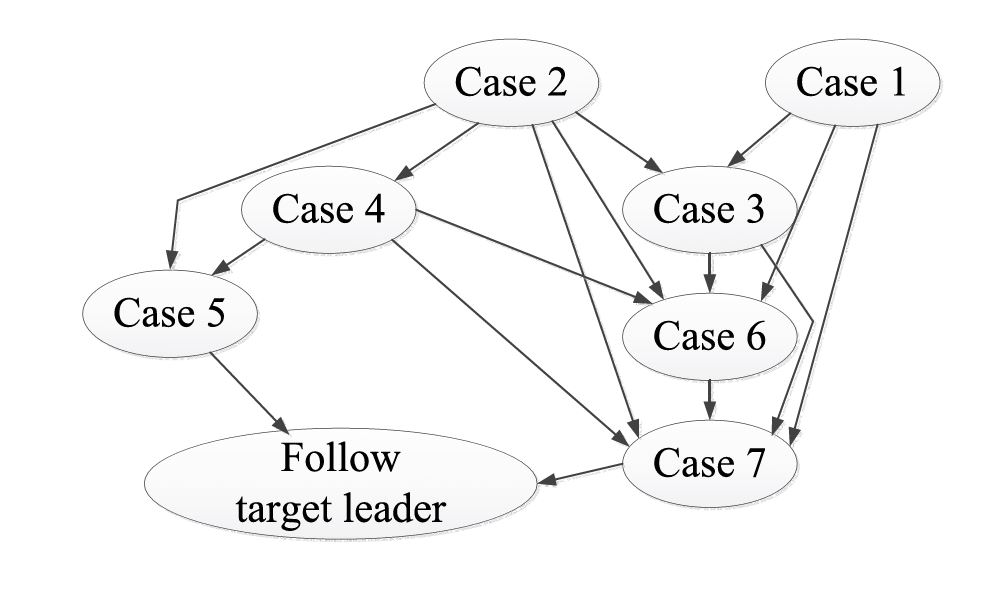
\includegraphics[width=\textwidth]{litReview/atagoziyevFlowchart.JPG}
\caption{The flowchart for Atagoziyev's Lane Changing model equations}
\label{fig:AtogoziyevFlowchart}
\end{figure}

Using this algorithm, we can move multiple vehicles into their correct lanes. LV always provides space to allow each changing vehicle into the correct lane. All of the vehicles are working with each other, such that they can all reach their goal.

\subsection{The MOBIL Model}
\label{subsec:The MOBIL Model}
The `Minimising Overall Braking Induced by Lane Changes' model defines two criterion that vehicles must satisfy. The first criterion deals with safety, ensuring that the deceleration of a successor vehicle $\tilde{a}_n$ in the target lane doesn't exceed a safety limit $b_{safe}$.

\begin{equation}
\tilde{a}_n \geq -b_{safe}
\end{equation}

This criterion effectively puts a limit on the level of braking a vehicle changing lanes can cause another vehicle to undergo if it pulls out in front of it.

The second criterion is the 'incentive criterion' which is what motivates a driver to change lanes. This criterion introduces a 'politeness factor' $p$ which expresses the extent to which nearby vehicles affect a driver's lane changing decision. 

The paper discusses the differences between symmetric ('US') lane changing rules and asymmetric ('European') passing rules. The US rules give the incentive criterion:

\begin{equation}
\underbrace{\tilde{a}_c - a_c}_\text{driver} + p(\underbrace{\tilde{a}_n  - a_n}_\text{new follower} + \underbrace{\tilde{a}_o - a_o}_\text{old follower}) > \Delta a_{th}
\end{equation}

$\tilde{a}_x - a_x$ is the utility a driver x gets due to the lane change, where $\tilde{a}_x$ is the acceleration of vehicle x after the lane change and $a_x$ was their acceleration before the lane change. $c$ is the vehicle changing lanes, $n$ is the vehicle behind $c$ once it changes lanes, and $o$ is the vehicle following $c$ before the lane change. $\Delta a_{th}$ is the threshold at which the driver will change lanes. It is designed to model inertia. A driver won't change lanes unless they get above a specific utility gain. The politeness factor $p$ varies from $0$ to $1$, where $p = 0$ is the most selfish behaviour and $p = 1$ describe drivers who won't change lanes unless collectively all of the drivers gain a utility greater than the threshold. When $p > 1$ drivers won't change lanes at all if it negatively affects the surrounding traffic, drivers will even go so far as to execute lane changes which reduce their own utility. Likewise drivers with $p < 0$ will go out of their way to negatively affect other drivers, even reducing their own utility to do so.

The idea of a MOBIL model means that drivers will only change when it increases the sum of all of the accelerations increases. This would be at $p = 1$ and $\Delta a_{th} = 0$. In this case the equation becomes 

\begin{equation}
\tilde{a}_c + \tilde{a}_n + \tilde{a}_o > a_c + a_n + a_o 
\end{equation}

\section{Merge Scenario Diagrams}
\label{sec:Merge Scenario Diagrams}
\begin{figure}[htb]
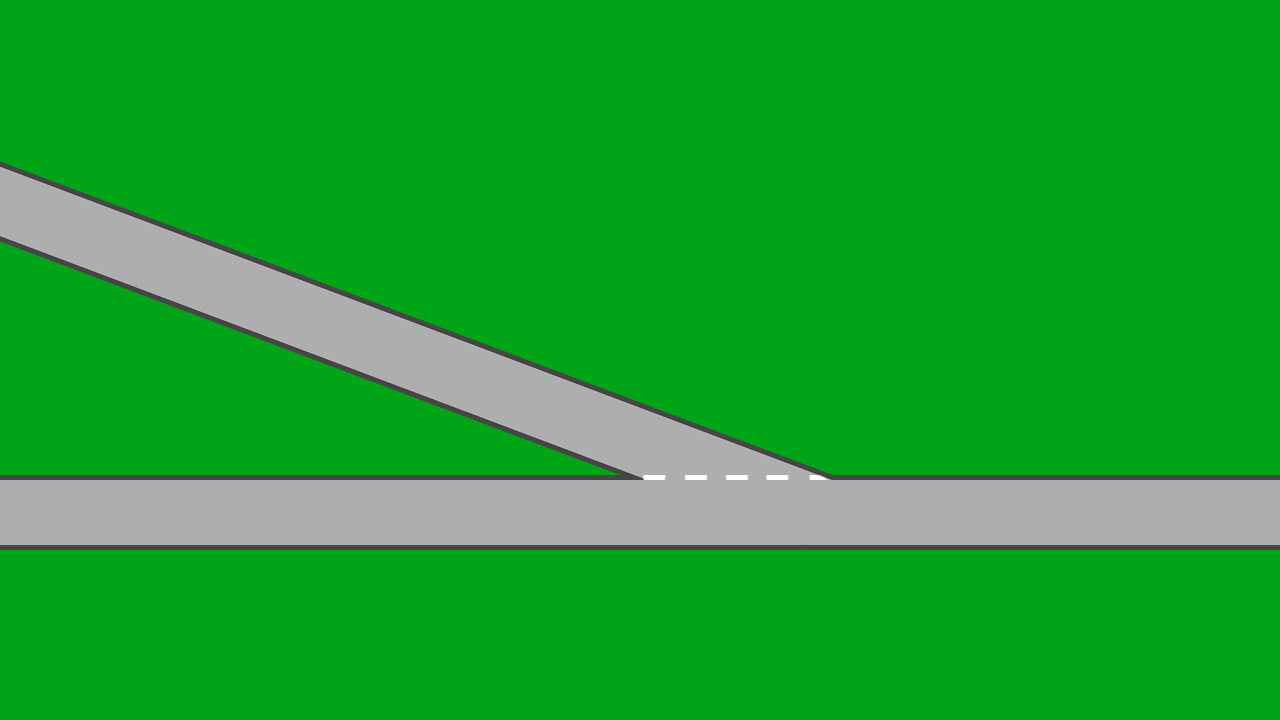
\includegraphics[width=\textwidth]{laneDiagrams/s2s.png}
\caption{A road with a single-to-single lane merge (S2S)}
\label{fig:S2SMerge}
\end{figure}

\begin{figure}[htb]
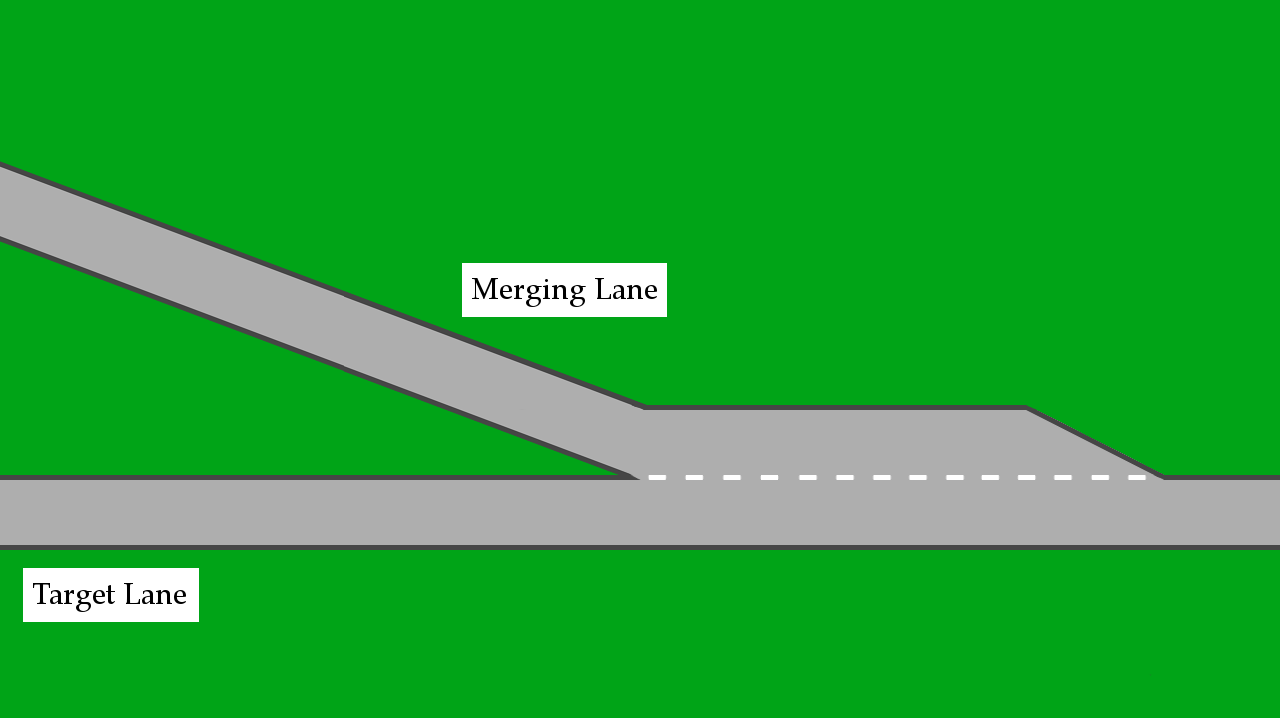
\includegraphics[width=\textwidth]{laneDiagrams/s2sExtended.png}
\caption{A road with a single-to-single lane merge and slip-lane (S2S)}
\label{fig:S2SMergeExtended}
\end{figure}

\begin{figure}[htb]
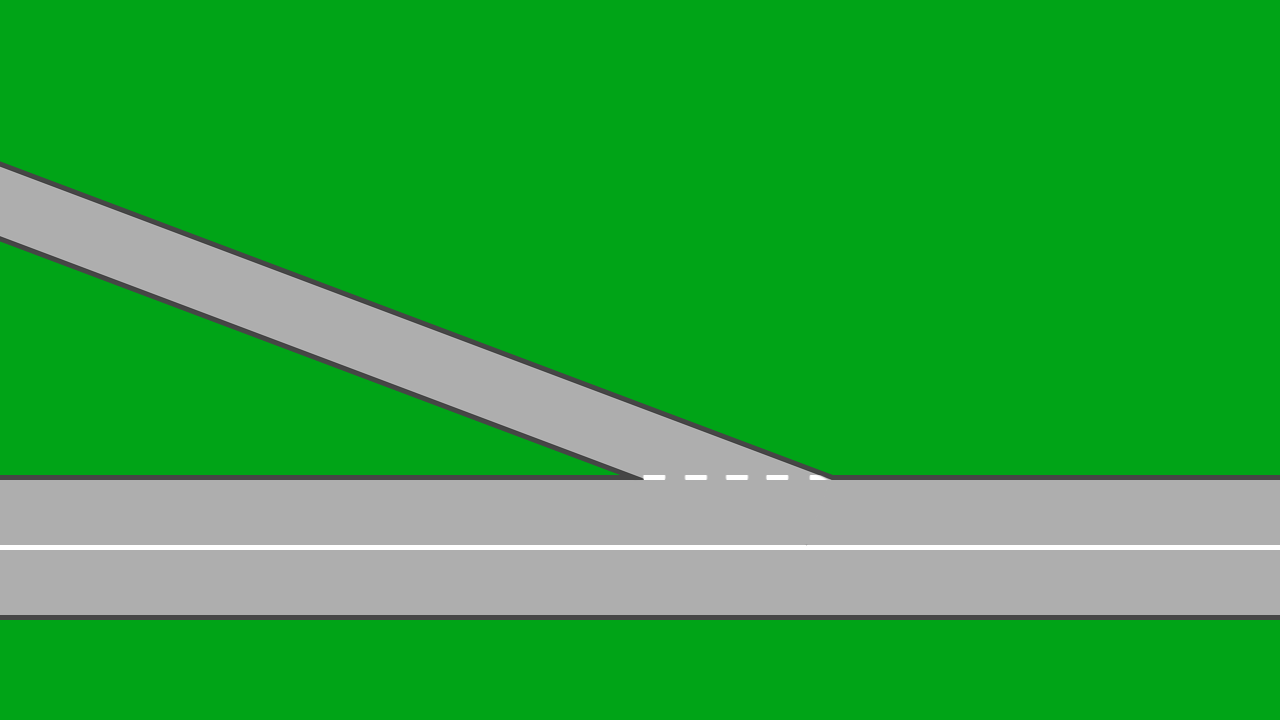
\includegraphics[width=\textwidth]{laneDiagrams/s2d.png}
\caption{A road with a single-to-double lane merge (S2D)}
\label{fig:S2DMerge}
\end{figure}

\begin{figure}[htb]
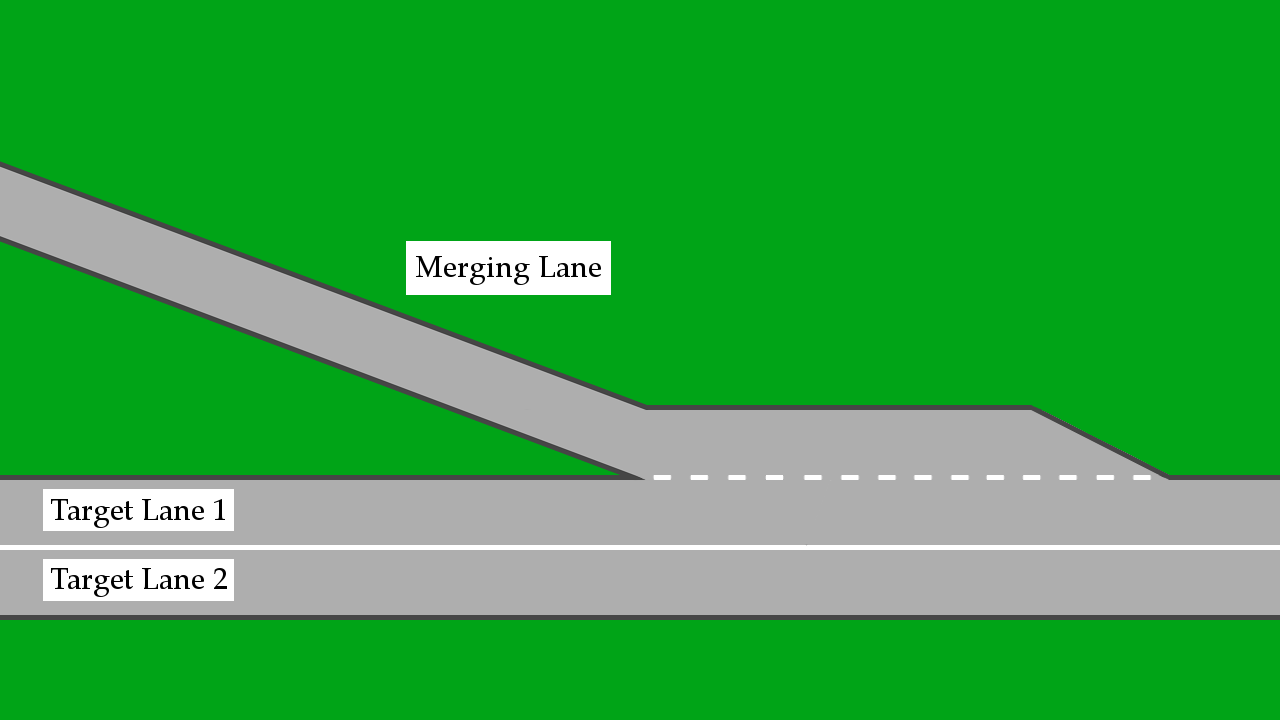
\includegraphics[width=\textwidth]{laneDiagrams/s2dExtended.png}
\caption{A road with a single-to{}-double lane merge and slip-lane (S2D)}
\label{fig:S2DMergeExtended}
\end{figure}

\begin{figure}[htb]
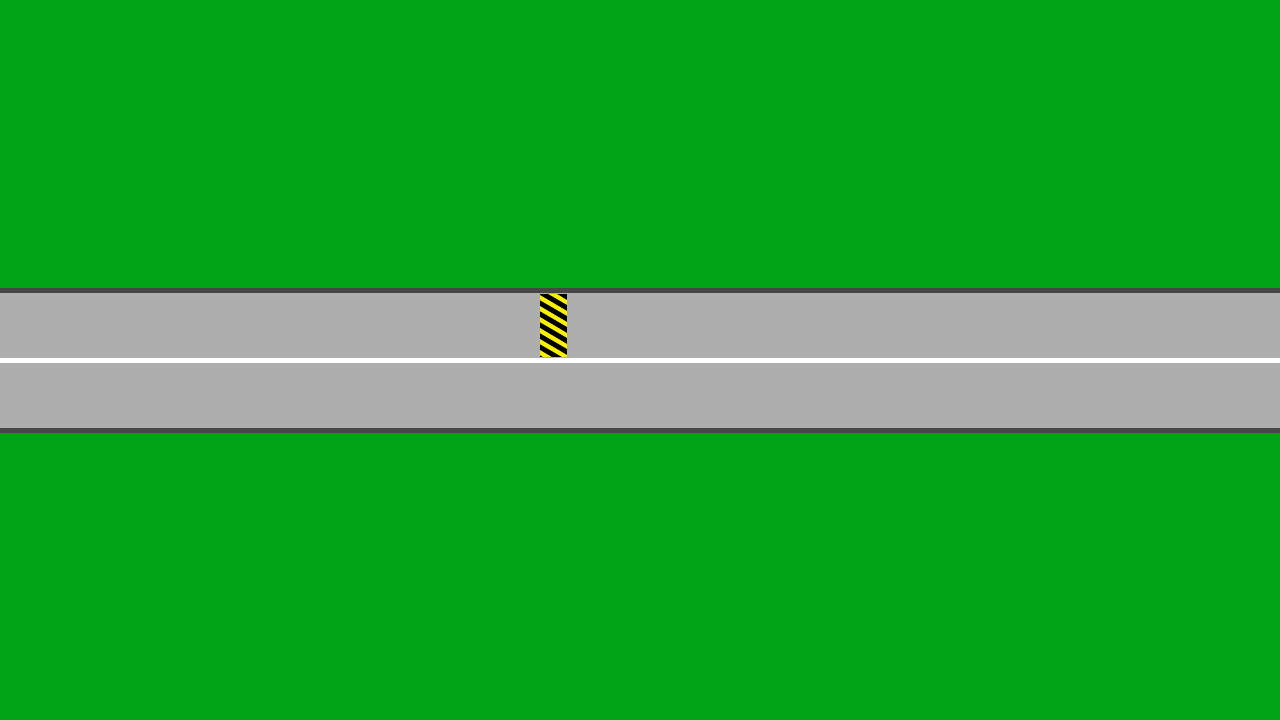
\includegraphics[width=\textwidth]{laneDiagrams/lane_blocker.png}
\caption{A road with a lane obstruction}
\label{fig:LaneObstruction}
\end{figure}

\section{S2S Map Calculations}
\label{sec:S2SMapCalculations}
To start with, we need to calculate the dimensions of the merging zone. The height of the merging zone will be the same as lane width of the target lane. The length can be calculated using the right-angled triangle in Figure \ref{fig:mergingZoneTriangle}. Using this triangle and some trigonometry we can calculate the length of the merge zone ($\text{mergingZoneLength}$ in Fig. \ref{fig:mergingZoneTriangle}) using equation \ref{hSin}.

\begin{figure}[htb]
\centering
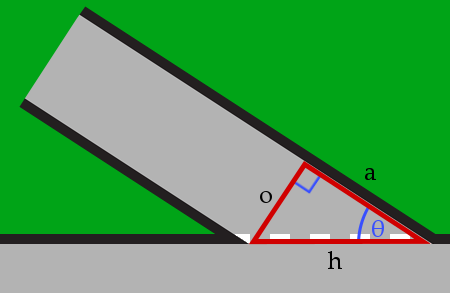
\includegraphics[width=10cm]{appendix/mergingZoneTriangle.png}
\caption{A right-angled triangle used to calculate the size of the merging zone.}
\label{fig:mergingZoneTriangle}
\end{figure}

\begin{equation}\label{hSin}
mergeZoneLength = \frac{laneWidth}{\sin(\theta)}
\end{equation}

We also need to know whether the horizontal width of the merge lane on the map, or it's 'base width' is longer than the target lane's lead in distance, plus the merge zone length. This will determine the width of the overall map, as if the merge lane's base length is longer then the target lane will not start with co-ordinate $x=0$ as it would if the target lane determined the width of the map.

Firstly we need to calculate the X and Y adjustments at the merge lane entrance. Because the vehicles drive in the centre of the lane and the merge lead in distance is defined by the middle line of the lane we still need to calculate how far the lane extends in the x and y directions due to it's width. To do this we can use the right-angled triangles shown in Figure \ref{fig:mergeEntranceTriangles}

\begin{figure}[htb]
\centering
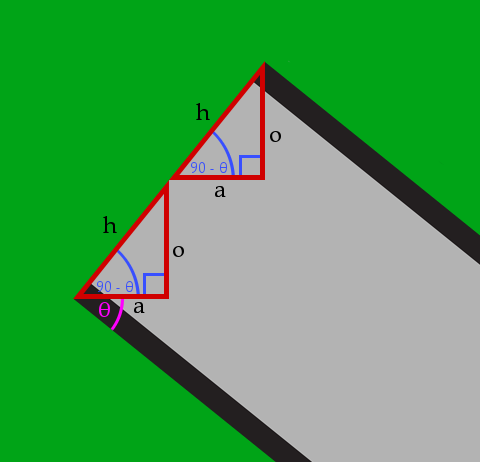
\includegraphics[width=10cm]{appendix/mergeEntranceTriangles.png}
\caption{Two right-angled triangles used to calculate the x and y adjustments for the merge entrance.}
\label{fig:mergeEntranceTriangles}
\end{figure}

These triangles have the same dimensions and have an interior angle of 90 - $\theta$ due to the 'alternate angle' or 'z-angle' rule. Each triangle has a hypotenuse with a length equal to half the width of the lane. 

The X-adjustment for the merge entrance is the length of the adjacent side of one of the lower triangle and the Y-adjustment for the merge entrance is the length of the opposite side of the upper triangle (though both triangles do have the same dimensions). We can use equation \ref{aCos90} to calculate the X-adjustment and equation \ref{oSin90} to calculate the Y-adjustment.

\begin{equation}\label{aCos90}
\text{x-adjust} = \frac{laneWidth}{2} \cos(90 - \theta)
\end{equation}

\begin{equation}\label{oSin90}
\text{y-adjust} = \frac{laneWidth}{2} \sin(90 - \theta)
\end{equation}

To calculate the 'base width' of the merge lane we will also need to calculate the adjacent side of the triangle in Figure \ref{fig:baseWidthTriangle}. In this triangle the hypotenuse has a length equal to the merge lead in distance. Therefore, we can use equation \ref{aCos} to calculate the length of the adjacent side. After obtaining the length of this side we simply add the merge entrance X-adjustment and half the length of the merge zone to find the merge base width.

\begin{figure}[htb]
\centering
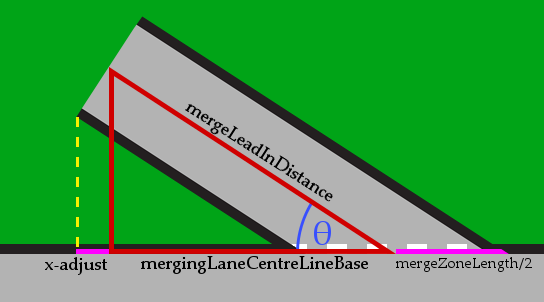
\includegraphics[width=10cm]{appendix/baseWidthTriangle.png}
\caption{A right-angled triangle used to help calculate the base width of the merge lane, along with the X-adjustment and merge-zone length.}
\label{fig:baseWidthTriangle}
\end{figure}

\begin{equation}\label{aCos}
mergingLaneCentreLineBase = mergeLeadInDistance \cos(\theta)
\end{equation}

We also need to find the point at which the merging lane's centre line crosses the target lane's centre line in the merge zone. We know the Y-coordinate for this point as it will be the same as the Y-coordinate of the target lane centre line. We also know the X-coordinate of the point at which the merge lane's centre line meets the target lane. We can use these two co-ordinates to create the triangle shown in Figure \ref{fig:toCentreTriangle}. We can then use equation \ref{aTan} to find the X-adjustment from the merge zone centre to the point where the two centre lines cross.

\begin{figure}[htb]
\centering
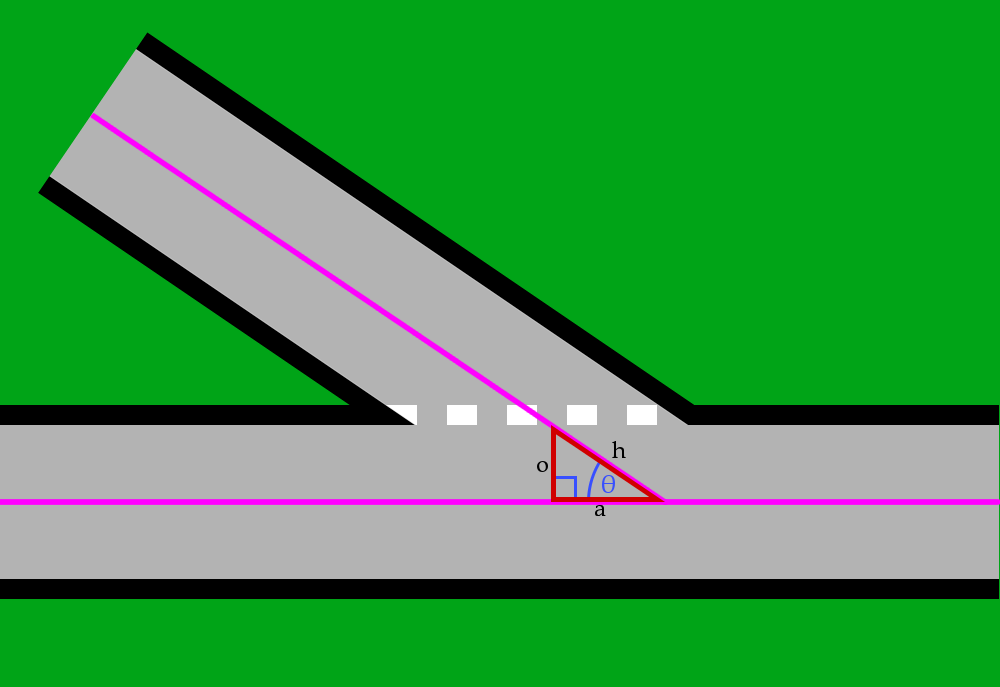
\includegraphics[width=10cm]{appendix/toCentreTriangle.png}
\caption{A right-angled triangle used to calculate where the two centre lines meet. The centre lines are indicated in pink.}
\label{fig:toCentreTriangle}
\end{figure}

\begin{equation}\label{aTan}
toCentreDistance = frac{laneWidth}{2 \tan(\theta)}
\end{equation}

\section{Generalising the Codebase}
\label{sec:Generalising the Codebase Appendix}
All class diagrams were created using the `IntelliJ IDEA 15.0.3' internal diagram tool. Figure \ref{fig:classDiagramKey} provides a key for understanding these diagrams.

\begin{figure}[htb]
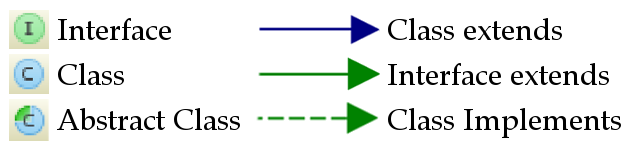
\includegraphics[width=\textwidth]{classDiagrams/classDiagramKey.png}
\caption{Key for the class diagrams in this report.}
\label{fig:classDiagramKey}
\end{figure}

\subsection{aim4.driver}
\label{subsec:aim4.driver}
\emph{aim4.driver} controls how a vehicle behaves on the map. In the original simulator the drivers were built to deal with 4-way intersections, with general functionality tied into the same class. You can see how this was done in Figure \ref{fig:driverBefore}.

\begin{figure}[htb]
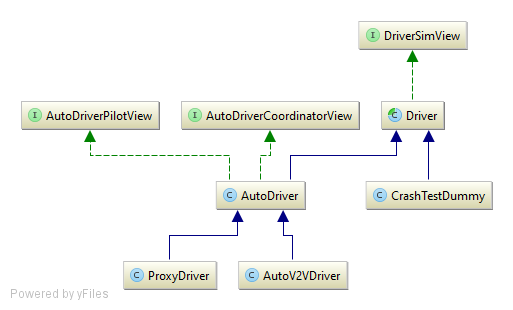
\includegraphics[width=\textwidth]{classDiagrams/driverBefore.png}
\caption{The original class structure for \emph{Driver}.}
\label{fig:driverBefore}
\end{figure}

The first major change was renaming \emph{DriverSimView}, \emph{AutoDriverPilotView}, and \emph{AutoDriverCoordinatorView} to end in \emph{Model} instead of \emph{View}. These interfaces are used to limit the methods that other classes can access in Driver and AutoDriver, thus changing their 'view' of that class. We felt that \emph{View} could cause confusion with the GUI elements of the simulator; we instead chose to refer to these interfaces as \emph{Models}, because the accessors are effectively given a model of Driver and AutoDriver (beyond which they care very little) that they can use to access methods.

The next change was separating out all of the AIM specific code into its own classes and interfaces. You can see how this was done in Figure \ref{fig:driverAfter} with \emph{AIMDriverSimModel} and \emph{AIMDriver}. The merge specific code found in \emph{MergeDriverSimModel}, \emph{MergeDriver} and \emph{MergeAutoDriver} is structured in a very similar manner to its AIM counterpart, taking advantage of the generalised code.

\begin{sidewaysfigure}[p]
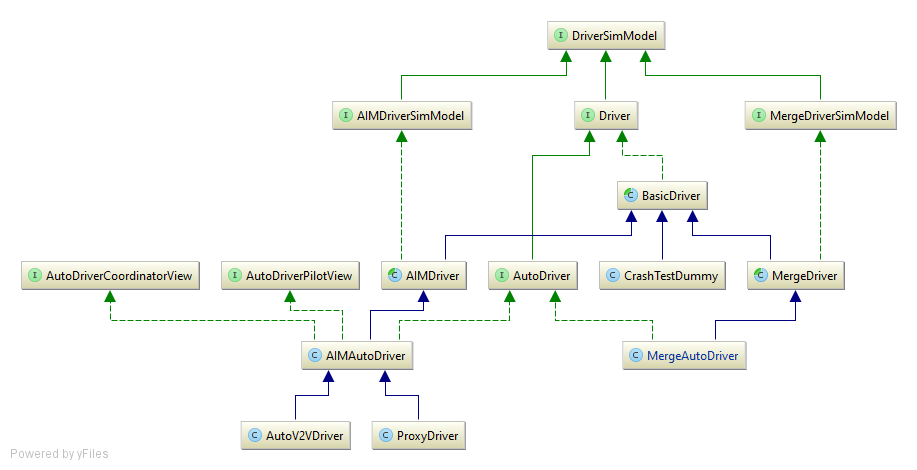
\includegraphics[width=\textwidth]{classDiagrams/driverAfter.png}
\caption{The new class structure for \emph{Driver}.}
\label{fig:driverAfter}
\end{sidewaysfigure}

As a consequence of breaking out the code like this, a number of additional changes had to be made. Driver was changed into an interface and a new class \emph{BasicDriver}. \emph{Driver} is simply used as an interface for accessing Drivers in non-simulation contexts (such as \emph{BasicVehicle}). \emph{BasicDriver} contains the generalised functionality all \emph{Driver} objects should need, with AIM specific activities moved to \emph{AIMDriver}. Extending from \emph{Driver} is the \emph{AutoDriver} interface, which adds no new methods but is instead used to categorise autonomous drivers. \emph{AIMAutoDriver} contains almost exactly the same code as the original \emph{AutoDriver} class.

\FloatBarrier
\subsection{aim4.gui}
\label{subsec:aim4.gui}
\emph{aim4.gui} controls the GUI for the simulator. We had to adjust this to allow for non-AIM simulations to be run. We chose to use tabs to allow users to switch between simulators (these are greyed out when a simulation is running). To make adding new tabs and simulation screens easier we had to refactor \emph{Viewer} into smaller, separate components. You can see the structural changes in Figures \ref{fig:originalAIMSetupLabeled} and \ref{fig:newAIMSetupLabeled}.

In the original simulator \emph{Viewer} displays the simulator set-up controls, \emph{SimSetupPanel}, and the simulation viewer \emph{Canvas} inside \emph{mainPanel}. \emph{mainPanel} is a \emph{JPanel} with a \emph{CardLayout} allowing the panel to switch between displaying the set-up controls and the viewer. In the new simulator we replaced \emph{mainPanel} with \emph{tabbedPane}, a \emph{JTabbedPane} object that allows users to switch between the different simulators using tabs. Each tab displays a \emph{SimViewer}, which behaves in a similar way to \emph{mainPanel} allowing users to switch between the set-up screen and the simulation screen using \emph{CardLayout}. Each simulator will have their own SimViewer type, as shown in Figure \ref{fig:simViewer}.

\begin{figure}[htb]
\centering
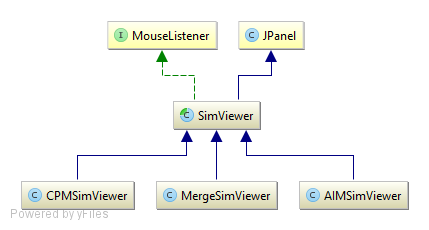
\includegraphics[width=8cm]{classDiagrams/simViewer.png}
\caption{The class diagram for \emph{SimViewer}.}
\label{fig:simViewer}
\end{figure}

We didn't want to force new simulators to use a full representation of vehicles on screen, as \emph{Canvas} does. To avoid this we created a new interface \emph{SimScreen} which \emph{SimViewer} uses to describe it's viewer card. Any class implementing \emph{SimScreen} can be used as the viewer for a simulation. Figure \ref{fig:simScreen} shows how \emph{MergeStatScreen} and \emph{Canvas} using \emph{SimScreen}.

\begin{figure}[htb]
\centering
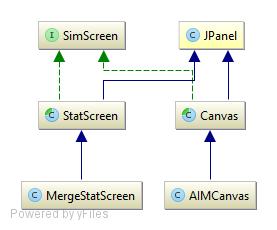
\includegraphics[width=8cm]{classDiagrams/simScreen.png}
\caption{The class diagram for \emph{SimScreen}.}
\label{fig:simScreen}
\end{figure}

We also generalised the \emph{SimSetupPanel} class to allow \emph{SimViewer} to display non-AIM set-up controls. Figure \ref{fig:simSetupPanel} shows the new class structure for \emph{SimSetupPanel}.

\begin{figure}[htb]
\centering
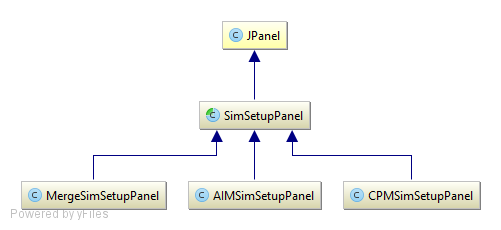
\includegraphics[width=8cm]{classDiagrams/simSetupPanel.png}
\caption{The class diagram for \emph{SimSetupPanel}.}
\label{fig:simSetupPanel}
\end{figure}

We also made a small adjustment to the behaviour of the reset option in the menu. Now the simulator must be paused in order for the reset button to be active. We did this because resetting the simulator without pausing was creating \emph{NullPointerException}s.

\begin{figure}[p]
\centerline{
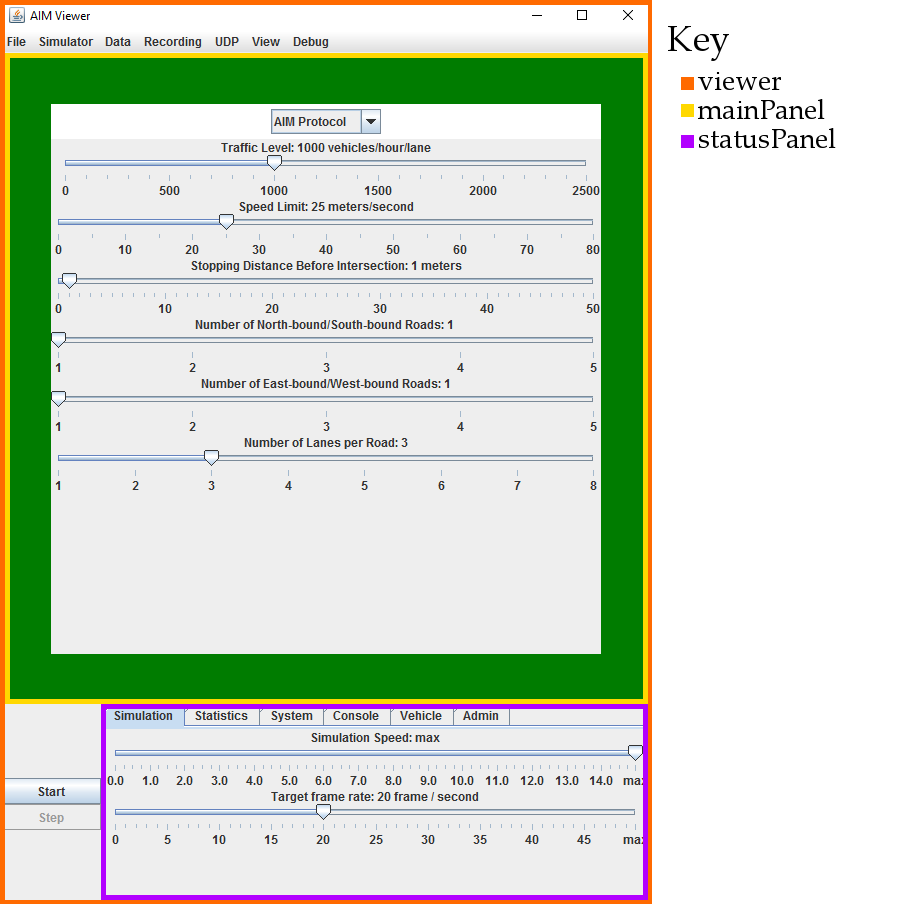
\includegraphics[width=15cm]{screenshots/originalAIMSetupLabeled.png}
}
\caption{Panel layout in the original simulator.}
\label{fig:originalAIMSetupLabeled}
\end{figure}

\begin{figure}[p]
\centerline{
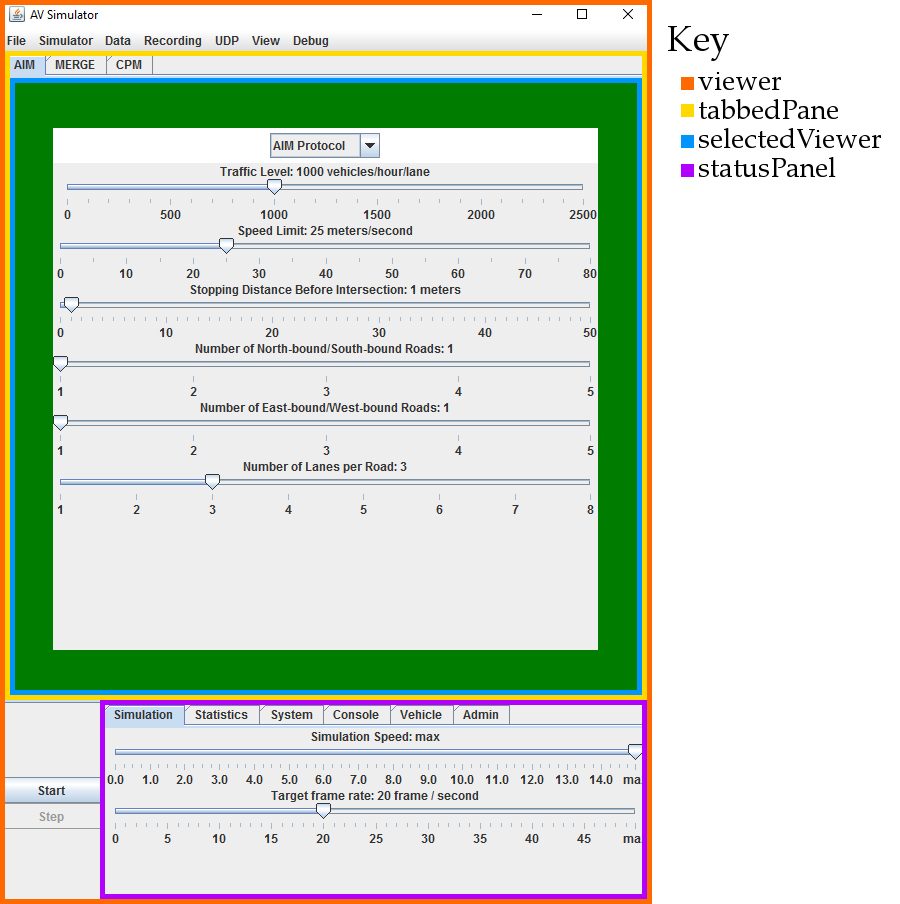
\includegraphics[width=15cm]{screenshots/newAIMSetupLabeled.png}
}
\caption{Panel layout in the new simulator.}
\label{fig:newAIMSetupLabeled}
\end{figure}

\FloatBarrier
\subsection{aim4.map}
\label{subsec:aim4.map}
\emph{aim4.map} is used to describe the environment vehicles are required to navigate. They also spawn vehicles that then drive through the map. Figures \ref{fig:mapBefore} and \ref{fig:mapAfter} show the original and new class structure for \emph{aim4.map}.

\begin{figure}[htb]
\centering
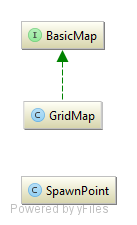
\includegraphics[height=6cm]{classDiagrams/mapBefore.png}
\caption{The original class structure for \emph{BasicMap} and \emph{SpawnPoint}.}
\label{fig:mapBefore}
\end{figure}

\begin{figure}[htb]
\centering
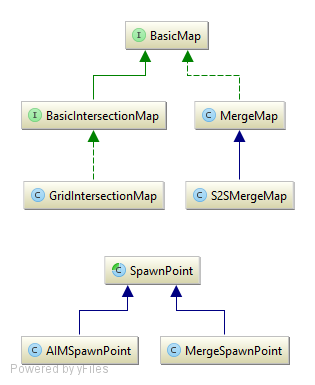
\includegraphics[width=8cm]{classDiagrams/mapAfter.png}
\caption{The new class structure for \emph{BasicMap} and \emph{SpawnPoint}.}
\label{fig:mapAfter}
\end{figure}

The changes made to \emph{aim4.map} were relatively straight-forward. The AIM specific features in \emph{BasicMap} were extracted out in \emph{BasicIntersectionMap} and \emph{GridMap} was renamed to \emph{GridIntersectionMap} and now inherits from the new interface. This allows for new map types, such as \emph{MergeMap} to implement a map type without AIM features.

\emph{SpawnPoint} was also broken out into general and AIM specific features. This had to be done because \emph{SpawnPoint} used to create \emph{SpawnSpec} objects with \emph{destination} fields. \emph{destination} is an AIM specific field relating to the intersection exit a vehicle plans to reach. By extracting this out new map types can spawn vehicles with \emph{SpawnSpec} instances specific to their map type.

\FloatBarrier
\subsection{aim4.sim}
\label{subsec:aim4.sim}
\emph{aim4.sim} contains the code responsible for constructing and running simulations. The original code was very focussed on AIM simulations and so we had to break the interfaces to allow for different types of simulators. 

\emph{Simulator} is an interface that new simulators need to implement. We decided to extract out some of the AIM specific features into \emph{AIMSimulator}. We also added an override to \emph{getMap()}, forcing AIM simulators to use \emph{BasicIntersectionMap} maps. The class structure changes can be seen in Figures \ref{fig:simulatorBefore} and \ref{fig:simulatorAfter}.

\begin{figure}[htb]
\centering
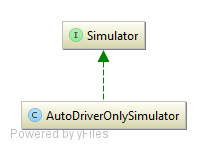
\includegraphics[width=8cm]{classDiagrams/simulatorBefore.png}
\caption{The original class structure for \emph{Simulator}.}
\label{fig:simulatorBefore}
\end{figure}

\begin{figure}[htb]
\centering
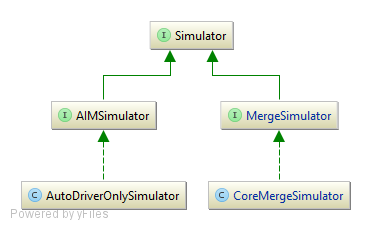
\includegraphics[width=12cm]{classDiagrams/simulatorAfter.png}
\caption{The new class structure for \emph{Simulator}.}
\label{fig:simulatorAfter}
\end{figure}

\emph{SimSetup} was also modified to separate AIM specific set-up options and simulator creation code from other simulators. Figures \ref{fig:simSetupBefore} and \ref{fig:simSetupAfter} show how these classes were altered.

\begin{figure}[htb]
\centering
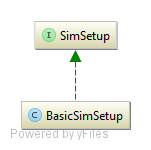
\includegraphics[height=6cm]{classDiagrams/simSetupBefore.png}
\caption{The original class structure for \emph{SimSetup}.}
\label{fig:simSetupBefore}
\end{figure}

\begin{figure}[htb]
\centering
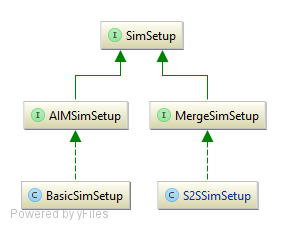
\includegraphics[width=10cm]{classDiagrams/simSetupAfter.png}
\caption{The new class structure for \emph{SimSetup}.}
\label{fig:simSetupAfter}
\end{figure}

\FloatBarrier
\subsection{aim4.vehicle}
\label{subsec:aim4.vehicle}
\emph{aim4.vehicle} controls the different vehicles used during simulations. Vehicles are used by both \emph{Driver} and \emph{Simulator} instances. To allow them to do that the original simulator code used \emph{View} interfaces similar to those in \ref{subsec:aim4.driver}. Figure \ref{fig:vehicleBefore} shows how these interfaces link together. Extracting AIM behaviour was quite difficult because of how interconnected these interfaces were. The solution we came up with was to create AIM specific interfaces and link them together in a similar manner, inheriting from the generic ones if possible. Figure \ref{fig:vehicleAfter} shows how the new structure links together.

\begin{figure}[htb]
\centering
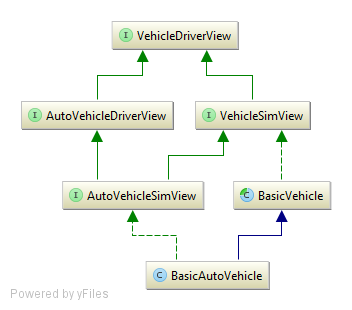
\includegraphics[width=10cm]{classDiagrams/vehicleBefore.png}
\caption{The original class structure for \emph{aim4.vehicle}.}
\label{fig:vehicleBefore}
\end{figure}

\begin{sidewaysfigure}[p]
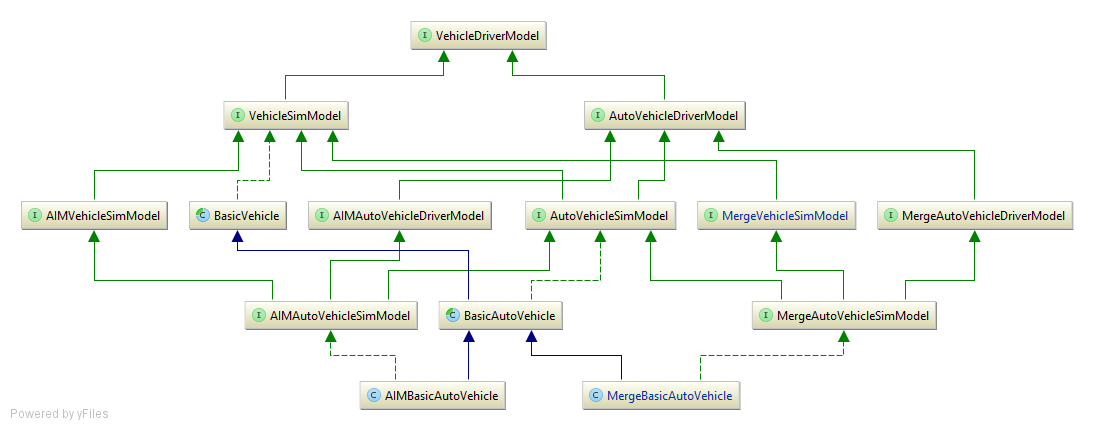
\includegraphics[width=\textwidth]{classDiagrams/vehicleAfter.png}
\caption{The new class structure for \emph{aim4.vehicle}.}
\label{fig:vehicleAfter}
\end{sidewaysfigure}

The first change made to \emph{aim4.vehicle} was to rename all of the files ending in \emph{View} to end in \emph{Model} instead. This matches the changes made to \emph{aim4.driver}.

\emph{AIMVehicleSimModel} and \emph{AIMAutoVehicleDriverModel} are at the top of the AIM interface tree. They both extend their generic counterparts. \emph{AIMAutoVehicleSimModel} extends these two interfaces along with \emph{AutoVehicleSimModel}. This matches up to the original inheritance structure. Any future vehicles will need to create their own version of these interfaces, as seen in \emph{MergeVehicleSimModel}, \emph{MergeAutoVehicleDriverModel} and \emph{MergeAutoVehicleSimModel}. 

In terms of classes we made \emph{BasicAutoVehicle} abstract and extracted out AIM specific behaviour to \emph{AIMBasicAutoVehicle}. \emph{BasicAutoVehicle} had to be abstract because we wanted to force \emph{getDriver()} to be overridden in subclasses to retrieve the simulator specific \emph{AutoDriver} for that vehicle (for example \emph{AIMAutoDriver} in AIM simulators). 

\FloatBarrier
\section{Maps}
\label{sec:Maps}
All maps testing Merge functionality implement \emph{BasicMap}. I created a generalised implementation called \emph{MergeMap} which satisfies the basic functionality of BasicMap as well as some protected accessors. All maps used during simulations extend \emph{MergeMap}.

\subsection{MergeMapUtil}
\label{sec:MergeMapUtil}
Similar to AIM's \emph{GridMapUtil}, \emph{MergeMapUtil} provides useful functions to \emph{MergeMap}, including \emph{SpawnPoint} \emph{VehicleSpec} generators.

\section{Merge Simulator Screenshot}
\label{sec:Merge Simulator Screenshot}
\begin{sidewaysfigure}[p]
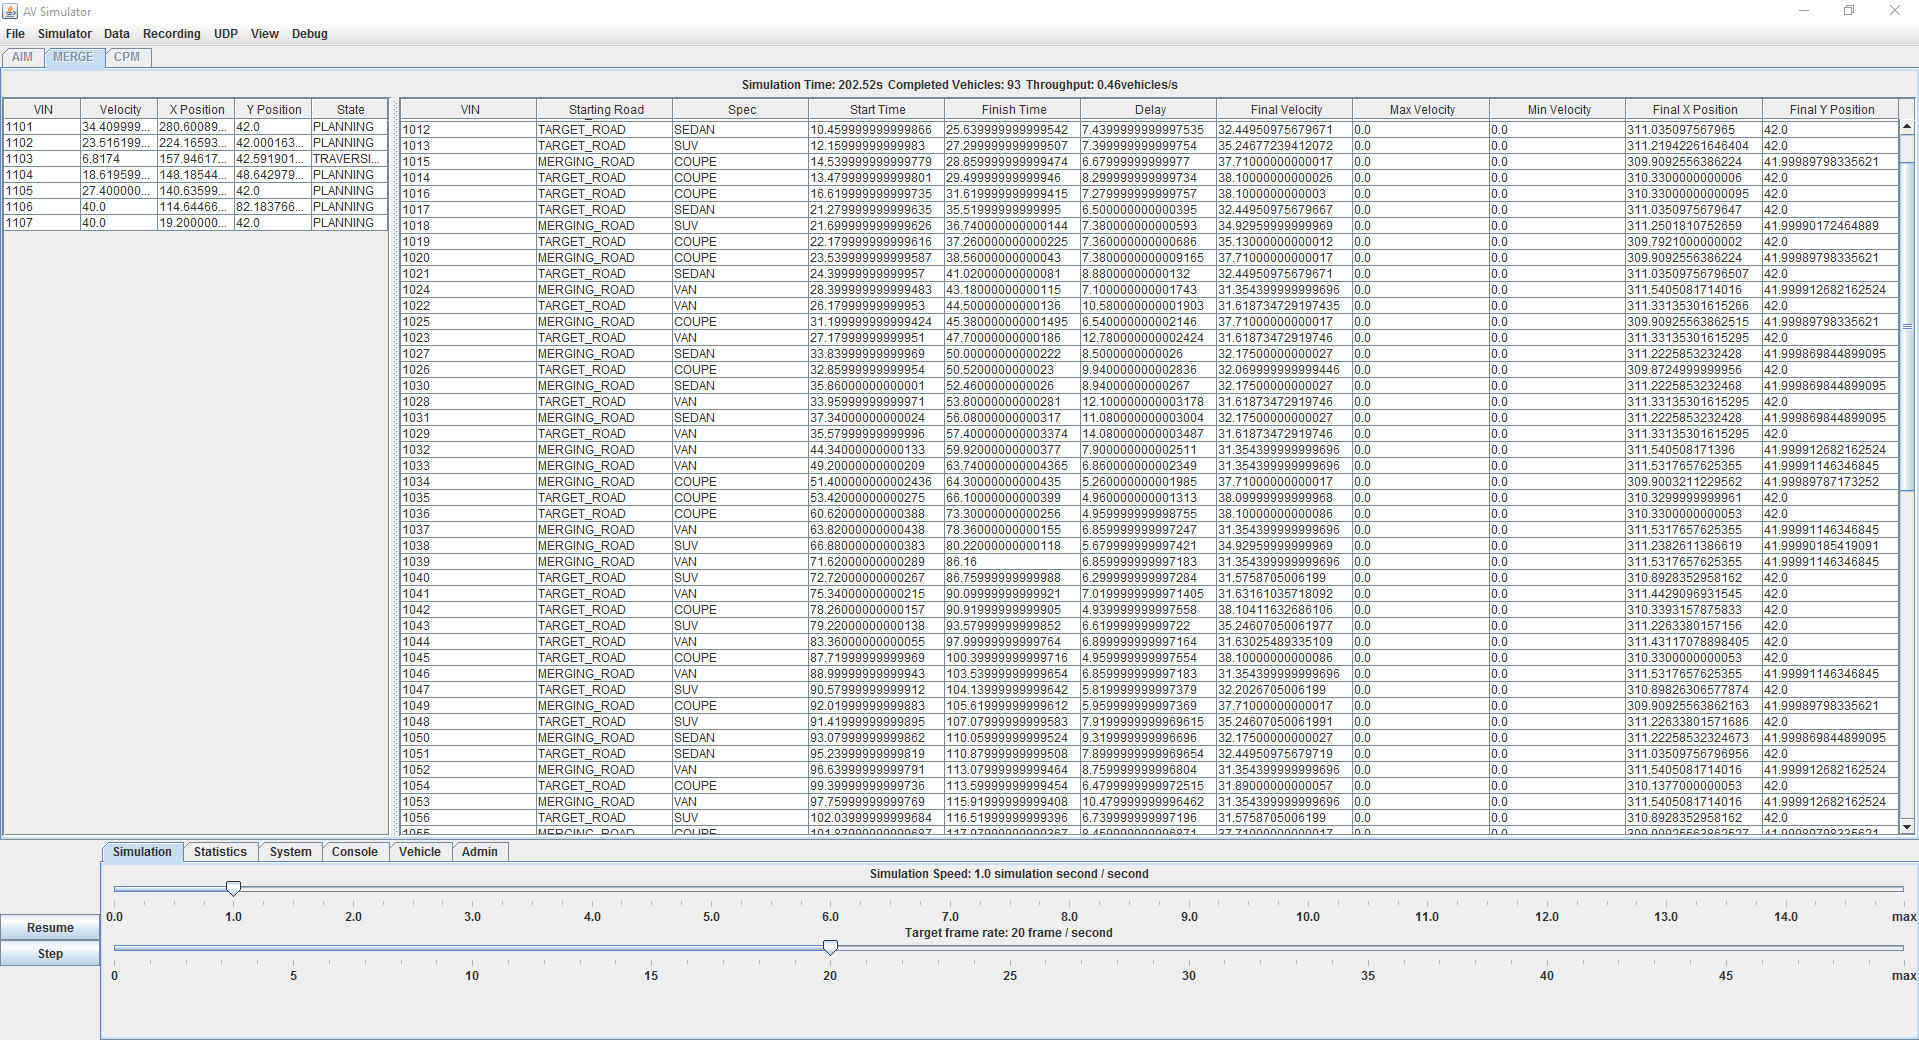
\includegraphics[width=\textwidth]{screenshots/s2sSimulationScreen.png}
\caption{The simulation screen for the S2S merge screen}
\label{fig:s2sSimScreen}
\end{sidewaysfigure}

\section{Lead in Distance Analysis}
\label{sec:Lead in Distance Analysis}
The lead in distance adjustments affect how long vehicles have to organise and communicate with QMM. Different lead in distance pairs were tested. The traffic rate was set to 1000\si{vhl}, the merge angle was set to 45\degree, and the speed limit was set to 20$\si{ms^{-1}}$ (44.7\si{mph} or 72\si{kph}).

Due to the 150\si{m} distance limit on requests, lead ins at 100\si{m} were worse for the lane with the 100\si{m} lead in. The only exceptions were when both lanes had lead in distances of 100\si{m}.

If one lane has a 100\si{m} lead, then the other lane also suffers a performance hit. This affect is most noticeable when the target lane has the 100\si{m} lead, but this effect is also seen with the merge lane. 

Beyond 150\si{m} the lead in distance had very little effect on the performance of the system. Throughput remained relatively constant throughout. Appendix \ref{fig:meanDelayLeadIn} shows how the mean delay relates to the lead in distance.

\begin{figure}[p]
\centerline{
	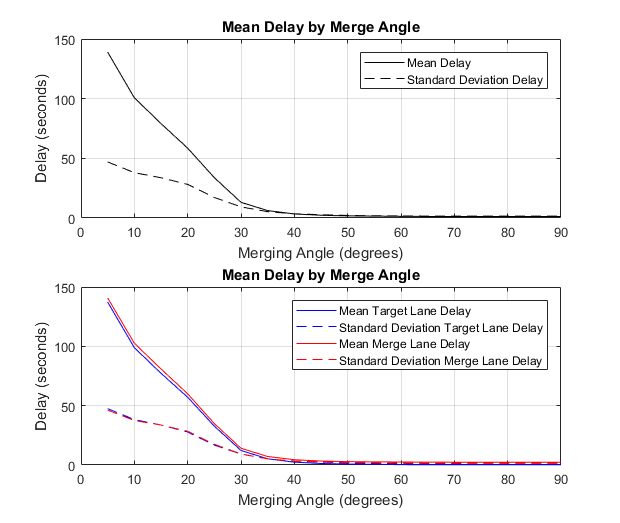
\includegraphics[height=\textheight]{plots/leadIn/meanDelay.png}
}
\caption{Bar chart showing mean delay by lead in distance}
\label{fig:meanDelayLeadIn}
\end{figure}


\end{appendices}